\chapter{Ludmila Zahradnik}

Ludmila tried to relax for a while before dealing with Jeeves – it didn’t work, of course, as her monumental pile of tasks pushed her to make any headway that she could. She made her way over to where the glossy black box was stuffed into the hold and pulled it back out again. There was no movement from within as she carried it back to her seat, nor could she hear the sound of the Skeleton’s voice. Whether it was because the spell cast on the box still held or he had finally stopped his nihilistic keening, she could not guess.

 

The sounds of her opening the box was the first indication that the Silence spell had expired, and the weak voice of Jeeves floated up as Ludmila looked down at the jumble of bones inside.

 

“Ah, the light – it burns so,” twin pinpoints of gleaming crimson light looked up at her. “Is it an angel: come to end my suffering…or is it a fiend: come to extend my torment?”

 

Ludmila resisted the urge to shake the box violently, she took a deep breath and tried to maintain a patient tone.

 

“I would like to speak with you,” she said. “Is it possible to discuss things calmly...or do I need to tie you to the mast?”

 

There was a long silence before the jumble of bones rose from the box, reassembling itself into its skeletal form. Jeeves stepped out and quietly sat down cross-legged on the deck, slouching despondently. Still, Ludmila was half-ready to spring up and grab the Skeleton should he attempt to drown himself again.

 

“The Royal Treasurer saw fit to assign you to me, Jeeves,” she said to him. “Have you been told the reason why?”

 

Jeeves’ eyes turned up from the deck, and his reply held as much energy as his posture.

 

“I only became aware of my own existence when you opened the box,” Jeeves shrugged. “Perhaps another one of me might know the answer to your question.”

 

“Another Jeeves?” Ludmila could not wrap her head around what he was saying, “Do you mean another Skeleton such as yourself?”

 

“I mentioned as much earlier, did I not?” He answered.

 

“So is your name Jeeves, or are you a type of Undead known as a Jeeves?”

 

The Skeleton stared at Ludmila, tilting his head in a way that very much suggested he thought there was something wrong with her.

 

“I am Jeeves,” he told her. “I am also called Jeeves. We are all Jeeves.”

 

His answer did absolutely nothing whatsoever to clear Ludmila’s confusion. Jeeves went on to explain at length.

 

“I am Jeeves,” he repeated himself, “as are all my kin. We are all Jeeves. Created in vast quantities and summoned for the convenience of our owners during their travels, adventures and conquests. It is supposed to be a temporary existence, but something has quite obviously gone very wrong.”

 

“So in this…temporary existence, you’re a merchant? You also said you refurbished equipment – does that mean you’re a smith as well?”

 

“Not just a smith, madam,” Jeeves replied. “I can repair any of your items, unless they have been completely destroyed. Your robes and staves; your swords and mail. Reimbursement for the cost of the repairs is a given, of course.”

 

“Of course…” Ludmila’s voice trailed off as she recalled what had happened when Aemilia tried to sell the basket, “but earlier, you acted as a merchant with no results.”

 

The points of Jeeves’ eyes went to the edge of the vessel again.

 

“Let’s put it to the test, shall we?” She quickly said to draw his attention back towards her, “I’ve some older clothing that has frayed a bit, I think.”

 

“I’ve mended all of your clothing, my lady,” Aemilia said. “Everything should be in good condition.”

 

Jeeves slouched further upon hearing her. Ludmila got up and fished around the hold until she finally decided to unroll the canvas holding her equipment and returned with it. Unsheathing the dagger at her hip, she cut a small slit in the fabric and held it out to Jeeves.

 

“Are you able to mend this?” She asked.

 

“I should be able to...” Jeeves replied hesitantly, taking the canvas and examining the damage.

 

Recalling that it required payment, she drew a pair of copper coins from her purse and handed them over as well. As with the exchange with the basket earlier in the day, a period of time passed and nothing happened. Jeeves looked back up from his task, and Ludmila half expected tears to come rolling out of his eye sockets. How could he be so expressive with no facial features to speak of?

 

“Aemilia, do you have a sewing kit?” Ludmila asked.

 

“Of course, my lady,” her maid replied. “Just one moment.”

 

Ludmila wasn’t sure why she had expected some fantastical thing to happen just because Jeeves claimed that it would. Aemilia returned and placed her sewing kit in front of the limp skeleton, who made a great show of looking depressingly lethargic as he opened it and looked over the contents. He eventually got to work, however, and the damage was stitched up neatly in short order. He lifted the sheet of canvas in front of him, turning it about and looking it over from different angles.

 

“I did it?” Jeeves’ voice was filled with disbelief. “I di–ahem, of course I did.”

 

He handed the tarp back to Ludmila, and she thought it looked workable. She held it out towards Aemilia for a more informed opinion. After her maid inspected the mended fabric and nodded, Ludmila turned back to Jeeves to see if his other claims were also founded on real skills. It took until late in the evening for them to finish but, by the end of it, she thought she knew what the mysterious Royal Treasurer had intended for Jeeves.

 

As she had suspected – after Jeeves had proven one of his claims by mending the canvas – he also possessed the ability to function much like a merchant of sorts. He was able to keep track of inventories, anticipate shortages and manage things much like one would run a store or a warehouse. His immediate usefulness to her was apparent, but he came with a variety of problems as well.

 

Unlike a merchant, his sense of value seemed horribly skewed. The first problem manifested when he didn’t seem to recognize any coinage aside from gold and, when she had shown him a gold trade coin, he didn’t recognize it as such. Perhaps the Sorcerous Kingdom came from another part of the world that used an entirely different system of currency, though she couldn’t imagine how far removed that would have needed to be with the vast trading networks that used the trade coins stretching across the region and even further across the continent.

 

Fortunately, he was able to quickly familiarize himself with the locally used currencies...yet his valuations remained the same. Ludmila had to slowly go over a long list of goods and correct him on each of them, lest he massively undercharge or underpay. The values were so far off for so many of them that she decided against using him as a general merchant for the village, just in case she had missed something and the discrepancies resulted in a loss of trust for her house as a whole.

 

Another problem was that Jeeves did not understand any written languages that she did. The resources provided by the administration were written in the script used by Re-Estize and Baharuth, and when she showed them to him he was completely oblivious as to their contents. She tried the written language of the Theocracy, Roble and the utilitarian script that traders used – which she admittedly was not entirely well versed in – but Jeeves did not understand any of it. He was able to quickly grasp the numbers that were used regionally, however, so she had hopes for him learning written language as well.

 

The matter of his ability to repair things was also still largely a mystery. Jeeves seemed to only consider equipment and various articles worn on one’s person as items to be repaired. When she asked about buildings and vehicles such as wagons or ships, he was oddly adamant that he could not perform such repairs, despite apparently having such a wide skillset. She couldn’t put those questions to the test immediately, so she shelved them for later.

 

Ultimately, Ludmila decided that, after he had learned the script used by the local populations in E-Rantel, Jeeves would be suitable for managing the general inventories of the village warehouse, as well as keeping track of shipments and helping out with organizing the labourers’ equipment. The previously suicidal Skeleton seemed ecstatic that Ludmila had found a place where he could be useful at all and happily retired back into his box to be called upon once again when they landed at Warden’s Vale.

 

She placed Jeeves back into the hold, pulling out her baggage to prepare for the night. Taking several blankets from the largest of them, they set about arranging their bedding for the night. Truth be told, there wasn’t much to be done as they were sleeping in the open hold – the most they could do was arrange their luggage about them and huddle together beneath the blankets in a bid for warmth. As it was still early spring, the air over the river would become icy cold as night fell.

 

Ludmila was accustomed to sleeping late, so she continued to work quietly with her back to the ship’s mast as the night fell over them. Beside her, Aemilia was aware that her mistress was still active and attempted to stay awake but, as the cozy warmth between them built up, she kept nodding off until all that could be heard from her was soft and steady breathing. Her lady’s maid had done remarkably well, considering that only a couple of days ago she would have probably jumped overboard at the first sign of the Undead. Ludmila wondered how the other nobles and their servants would fare in the weeks to come, and if they too would be assigned Undead assistants.

 

Considering Jeeves’ confusing sense of identity, she thought it was bound to become a gigantic mess. He had mentioned that his ‘kind’ was created in vast quantities, so perhaps every noble and merchant in the realm would end up with a Jeeves of their own. In addition, there would eventually be hundreds of thousands of nameless Skeletal labourers, and thousands of Soul Eaters, Liches and Death Knights across the duchy.

 

“Don’t tell me you all have the same name as well,” Ludmila idly said to the Elder Lich as she continued her work.

 

It was still standing at the bow of the ship, facing away from her to watch the river ahead of them, yet it somehow knew it was being spoken to rather than any of the other Undead on the ship. It turned around and walked over to the open hold where the two women were resting.

 

“Such things are unnecessary,” it said while looking down at her with its glowing crimson gaze. “Even without names we know who is addressing us, and who is being addressed.”

 

“Even when there are thousands of nameless Undead in an area?”

 

“The number matters not.”

 

Despite its statement, it still didn’t feel right when someone worked closely with her. She couldn’t very well go on indefinitely saying ‘hey you,’ or ‘Elder Lich’ whenever she wanted to speak to her attaché – well, technically Ludmila supposed that she could, but it still didn’t sit well with her personally.

 

“Don’t you want a name?” She asked, “At the least, it would make things smoother when communicating with the citizens.”

 

At least she thought it would. Whether the sense of familiarity in knowing someone by name would overcome the idea that they were the Undead that were commonly known to hate the living was another question entirely. The Elder Lich did not respond, much like it did when it could not find a satisfactory answer to other questions she had asked in the past. Ludmila decided that it was as close to a ‘yes’ as she was going to get.

 

“Is there something that distinguishes you from the others? A trait or accomplishment you’re proud of, perhaps?”

 

After a pause that seemed so long that Ludmila thought she was not going to receive an answer, the Elder Lich spoke.

 

“I am the ninth of my kind to be trained under the Guardian Overseer as an administrative official for the E-Rantel civil authority.”

 

Ludmila was really hoping for a more colourful story. Did such powerful beings really lead such a mundane existence? Something else occurred to her as she thought on his words.

 

“Wait, does that mean that the Elder Liches in the civil office are the first eight?”

 

“Yes.”

 

The powerful and mystical realm of the Sorcerous Kingdom was getting more plain by the second. She supposed it was just from her own perspective as someone who was exposed to the underlying workings of the realm. The nobility was often portrayed in ludicrous and absurd ways by the common folk as well, and most of what she did was paperwork and routine border patrols. On the other hand, Jeeves certainly reacted with great enthusiasm upon finding out he would have a job, so perhaps all Undead servitors saw things the same way.

 

“The ninth administrator...ninth…” she murmured.

 

“That name is already taken,” her attaché said. “By another creation.”

 

“Truly?”

 

That the Sorcerous Kingdom had names that used numbers made things much easier, and inspiration immediately came to Ludmila’s mind.

 

“Then…what about Nonna?”

 

She looked up to the Elder Lich, who was silent for a moment. Then, it nodded slowly.

 

“This is acceptable.”

 

Though it had said as much, its voice seemed to carry a hint of hesitation. Ludmila was too pleased with her clever choice to pay it any mind, however. She decided to retire for the night with her small win, and settled herself more comfortably into her makeshift bedding beside Aemilia.

 

“Good night, Nonna.”

 

Nonna did not reply.


\begin{figure}
    \centering
    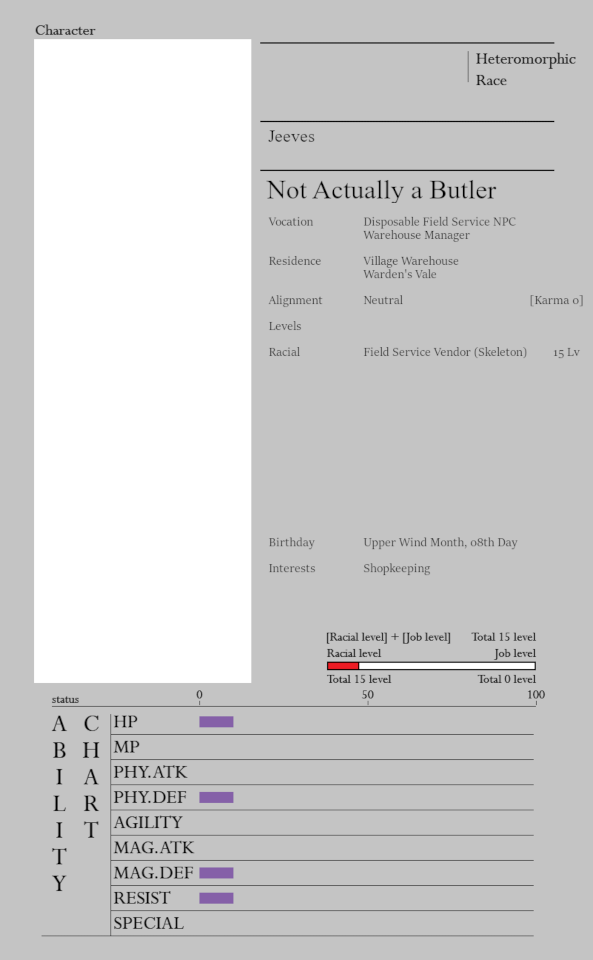
\includegraphics[width=1\textwidth]{images/b3h4A7o.png}
    \caption*{Jeeves Character Sheet}
\end{figure}

\section*{The Noble Household (Part III) – On Manservants}

As the female servants of the noble household are divided into many specific roles, so too are the men.

 

The quintessential manservant most commonly associated with male household staff, the Butler has its humble roots as a servant responsible for the management and serving of alcoholic beverages. Over time, they have grown into their more well known role of stewardship over the household and their responsibilities in leading the male household staff. A Butler is a senior member of the Household, usually reporting to the Lady of the House.

 

The Valet is the male equivalent of a Lady’s Maid, personally attending to the Lord of the House in much the same way his female counterpart attends to the Lady of the House. Large, affluent households may also employ valets for the adult male children of a noble family – particularly for the heir apparent of a great house or the princes of royalty.

 

Footmen are the highest ranking members of the junior household staff, serving as escorts, heralds, doormen, convenient muscle and attendants at a noble family’s meal. They may also serve in the capacity of a Valet to male members of a noble family or visiting guests. Arrays of tall, young and handsome footmen are as much a show of prestige and wealth as beautiful, young maids.

 

Pages were generally boys employed as couriers and attendants to nobles – both men and women – in the same way a Squire may attend to a Knight or Paladin and accompany them to battle.

 

Various other roles in the junior household staff are filled by men, and they are usually called by those specific duties(eg. A boot boy is responsible for taking care of footwear). As with female members of the kitchen staff, men that work in the kitchen report to the Cook.